\section{World Action Models}

The previous sections review world models as predictive models of the world: given the current observation or state and an action, they estimate how the world may evolve. In embodied decision making, however, prediction alone is not sufficient. A robot must also infer which actions can realize a desired future. This motivates an action-oriented extension of world models, which we refer to as \emph{world action models}. In this section, we use the term world model in a narrower sense: it refers to a language-conditioned video prediction model that generates future observations from the current observation and a high-level language instruction,
\[
o_{t+1:t+H} \sim p_\theta(\cdot \mid o_t, l),
\]
where $l$ denotes a language instruction and $o_{t+1:t+H}$ denotes a sequence of predicted future observations. A world action model further aims to connect such predicted futures with executable robot actions. Ideally, it models not only what the future should look like, but also how the robot should act to realize that future:
\[
(o_{t+1:t+H}, a_{t:t+H-1})
\sim p_\theta(\cdot \mid o_t, l).
\]
From this perspective, a world action model can be viewed as a bridge between visual future prediction and embodied control. Existing approaches differ in how they couple video prediction with action prediction. We organize them into four representative paradigms, as summarized in Fig.~\ref{fig:wam}.


\paragraph{Imagine-then-execute.}
The most direct paradigm is a two-stage \emph{imagine-then-execute} formulation ~\cite{unipi,susie,wen2024atm,liang2024dreamitate,avdc,feng2025vidar,gvftape,RIGVid}. In the first stage, a language-conditioned world model is used as a visual planner to generate future observations,
\[
o_{t+1:t+H} \sim p_\theta(\cdot \mid o_t, l).
\]
In the second stage, a separate inverse dynamics model or goal-conditioned policy maps the current observation and a predicted visual subgoal into robot actions,
\[
a_t \sim q_\phi(\cdot \mid o_t, \hat{o}_{t+1}).
\]
The two modules together form a world action model: the video model imagines a possible future, and the inverse dynamics model grounds this future into executable actions. This decomposition has several practical advantages. Since the visual planner and the action grounding model are separated, they can be trained on different data sources: the video model can benefit from large-scale visual data, while the inverse dynamics model can be trained on robot trajectories with action labels. The modular design also allows additional structure to be injected into the action grounding process. For example, one can estimate intermediate quantities such as end-effector poses ~\cite{gvftape, liang2024dreamitate}, object poses ~\cite{RIGVid}, or dense optical flow ~\cite{avdc} from the generated video, and then use these cues to derive or guide the corresponding robot actions. This decomposition provides flexibility, but it also makes action prediction dependent on the quality of the generated visual subgoals. Errors in the predicted subgoals may propagate to the inverse dynamics model, causing the predicted actions to deviate from the intended task execution.


\paragraph{Video-feature-conditioned action prediction.}
A second paradigm keeps the two-stage structure but does not require the video model to generate a complete future observation sequence ~\cite{videopolicy,hu2025vpp,ma2026dit4dit,pai2026mimicvideo}. This design is motivated by the computational cost of diffusion-based, where producing full future frames may require multiple iterative sampling steps. Instead of decoding a complete video rollout, these methods extract intermediate spatiotemporal features from the video prediction model and use them to condition an action prediction module:
\[
f_t = \mathcal{H}\big(u_\theta(o_t, l)\big),
\qquad
a_t \sim q_\phi(\cdot \mid o_t, f_t),
\]
where $u_\theta$ denotes the neural backbone of the video prediction model, $\mathcal{H}(\cdot)$ denotes a feature extraction operation, and $f_t$ denotes the extracted spatiotemporal representation. The underlying assumption is that the internal representations of a video model already contain useful information about task intent, scene dynamics, and possible future evolution, even if the model does not explicitly decode the final video during policy inference. This can substantially reduce inference cost compared with full video generation, while still transferring predictive visual representations to the action model. The main limitation is that the interface between the video model and the policy becomes a latent feature rather than an explicit visual plan. As a result, the intermediate representation is less interpretable, harder to inspect, and may not expose whether the policy is using meaningful future information or merely exploiting task-correlated features.

\begin{figure*}[t]
\centering
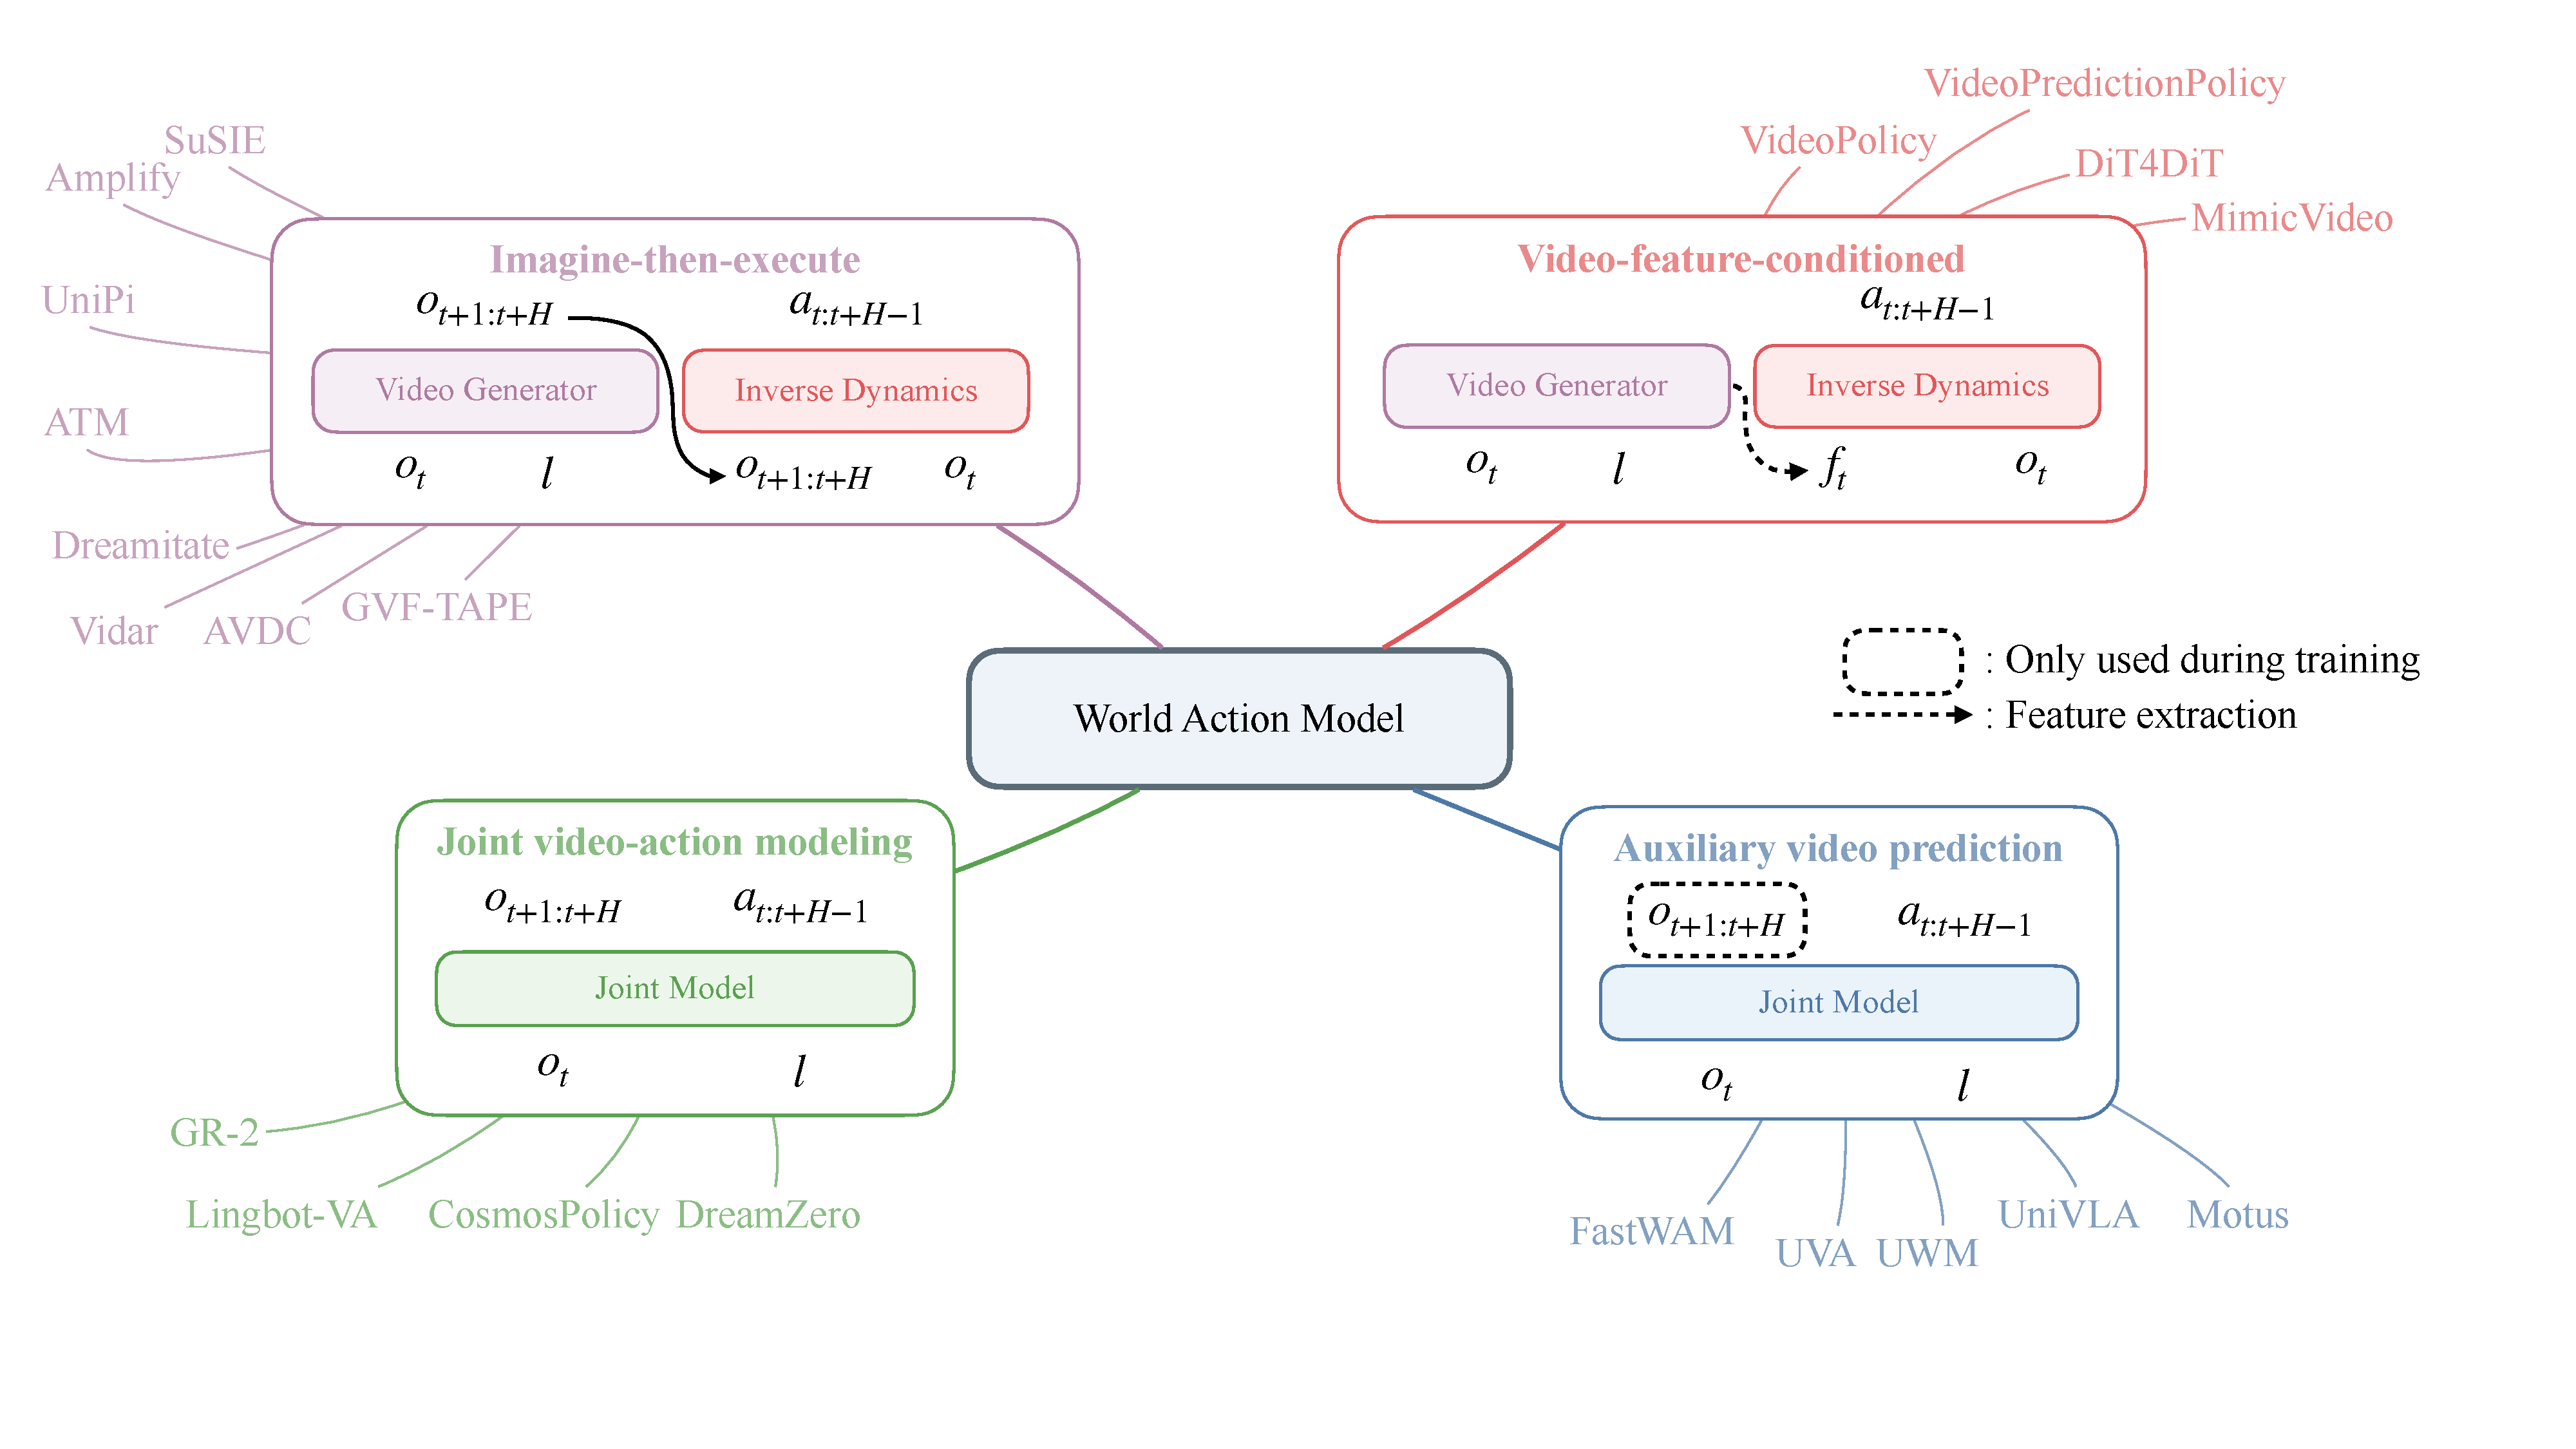
\includegraphics[width=0.95\linewidth]{figs/wam.pdf}
\caption{
Taxonomy of world action models.
Given the observation $o_t$ and language instruction $l$, world action models couple future observation prediction with robot action generation in different ways.
Representative paradigms include imagine-then-execute, video-feature-conditioned action prediction, joint video-action modeling, and auxiliary video prediction for policy learning.
}
\label{fig:wam}
\end{figure*}


\paragraph{Joint video-action modeling.}
A third paradigm attempts to model future observations and robot actions jointly within a single generative model ~\cite{ye2026dreamzero,kim2026cosmospolicy,cheang2024gr2,li2026lingbotva}:
\[
(o_{t+1:t+H}, a_{t:t+H-1})
\sim p_\theta(\cdot \mid o_t, l).
\]
In this formulation, video prediction and action prediction are not treated as two separate modules. Instead, the model learns a joint distribution over visual futures and the corresponding action sequences. A common strategy is to start from a video generation backbone pretrained on large-scale visual data ~\cite{cosmos,wan2025}, modify the architecture or output space so that it can also produce robot actions, and then adapt the model on robot trajectories with action labels. This unified formulation has the advantage that future observations and actions are learned in a shared representational space, which can improve their consistency: the generated actions are trained together with the visual future they are supposed to induce. However, joint modeling also inherits the difficulties of both video generation and action learning. It requires robot data with action labels for adapting the action output, and such data are much scarcer than ordinary videos. In addition, the model must jointly handle high-dimensional visual generation and precise action prediction, whose optimization objectives may not always be aligned. 

\paragraph{Auxiliary video prediction for policy learning.}
A fourth paradigm uses video prediction as an auxiliary training objective rather than as an explicit inference-time module~\cite{yuan2026fastwam,zhu2025uwm,li2025uva,bu2025univla,bi2026motus}. In this setting, the policy is trained with an additional prediction branch that reconstructs or generates future observations from the policy's internal representation. The purpose of this branch is not to produce an explicit visual plan for execution, but to encourage the policy backbone to encode spatiotemporal information related to future scene evolution. During training, the video prediction loss provides an auxiliary supervisory signal in addition to the action prediction loss. During inference, the auxiliary video branch can be removed, and only the action prediction head is used. This design avoids the cost of generating videos at test time while still using future prediction to shape the learned representation. Its limitation is that the predicted future is not explicitly used as a plan during execution. Therefore, the benefit of the video objective depends on whether the auxiliary prediction task induces representations that are useful for action selection. Balancing the action loss and the video prediction loss can also be nontrivial, since accurate visual prediction does not necessarily lead to better control.



Overall, these four paradigms represent different ways of coupling world prediction with action generation. Imagine-then-execute methods provide modularity and interpretability, but may suffer from a visual-action grounding gap. Feature-conditioned methods reduce the computational cost of explicit video generation, but sacrifice the transparency of visual plans. Joint video-action models offer a unified formulation, but require action-labeled robot data and must jointly optimize visual and action prediction. Auxiliary prediction methods improve efficiency at inference time, but rely on the training objective to implicitly transfer predictive information into the policy. The central design trade-off is therefore how explicitly the future should be represented and how tightly this future representation should be coupled with action prediction.
